% Created 2021-08-19 Thu 09:20
% Intended LaTeX compiler: pdflatex
\documentclass[11pt]{article}
\usepackage[utf8]{inputenc}
\usepackage[T1]{fontenc}
\usepackage{graphicx}
\usepackage{grffile}
\usepackage{longtable}
\usepackage{wrapfig}
\usepackage{rotating}
\usepackage[normalem]{ulem}
\usepackage{amsmath}
\usepackage{textcomp}
\usepackage{amssymb}
\usepackage{capt-of}
\usepackage{hyperref}
\author{Filipa  Calado}
\date{\today}
\title{}
\hypersetup{
 pdfauthor={Filipa  Calado},
 pdftitle={},
 pdfkeywords={},
 pdfsubject={},
 pdfcreator={Emacs 26.2 (Org mode 9.1.9)}, 
 pdflang={English}}
\begin{document}

\tableofcontents

\section{two}
\label{sec:orgdf26277}
\subsection{chapter overview}
\label{sec:org1581e8f}
\subsection{introduction}
\label{sec:org7c51c8a}

This chapter explores how to use TEI in order to work with queerness
in literary data. In this case, the literary data consists of a
manuscript of \emph{The Picture of Dorian Gray} by Oscar Wilde.

I examine how Wilde edited out suggestions and insituations of
homosexuality during the revising process of this manuscript.

I propose a method for marking these alterations and deletions in TEI
formal language. My customization \ldots{} 

\subsection{textual scholarship}
\label{sec:org96ad1bd}
\subsubsection{history of textual scholarship}
\label{sec:org472d4bc}
Before proceeding with the content of Wilde's manuscript, I will give
a general overview of editorial approaches in the field of Textual
Scholarship. Textual Scholarship is a generalized term that describes
the studying, annotating, and editing of textual materials like
manuscripts and books. Within this field, the branch of Textual
Criticism focuses specifically on identifying and analyzing variants
of manuscripts and books. Textual Critics often examine textual
variants in order to select an ideal witness to form the basis of a
Critical Edition.

The project of selecting an "ideal" witness creates some controversy
about the proper role and purview of the textual critic. Dominant
editorial practices increasingly delimit the purpose and purview of
the editor as a recoverer or preserver of texts, while other
perspectives permit the authority of the editor as an enabler of
textual readings. The history of Textual Criticism thus presents an
arc, which first tends toward what I call the "restorative approach"
then, with the advent of digital technology, the "productive
approach." With the popularization of digital tools, editing becomes
less about "correcting" or aligning text with a prior witness, and
more about finding ways to multiply the text's potential forms and
readings. As I review the different approaches, I emphasize how the
\emph{productive} capacity functions within textual editing paradigm. I
will look to ways that editorial pracitices have opened up a space for
the editor's role as a content \emph{creator} rather than recoverer.

The "restorative approach" begins with the work of Ronald B. McKerrow,
a leading twentieth-century Shakespearean scholar, who maintains that
the goal of textual criticism to preserve authorial
intention. McKerrow proposes an influential model for "copy-text"
editing, which establishes the base text for editing (the "copy-text")
on an early witness that most closely resembles the author's original
intention. During the editorial process, the editor defers to this
early text in order to settle differences among variants.

Though highly influential, McKerrow's approach creates its own
resistance among textual scholars, who decry the "the tyranny of the
copy-text" that prevents them from drawing on other textual
variants. To address these concerns, Walter W. Greg's work, \emph{The
Rationale of Copy-Text} proposes that critics use the copy-text as a
basis for accidental elements like spelling and punctuation, while
expanding their purview of substantive elements to other witnesses
that may contain changes by the author.\footnote{Greg, Walter W. "The Rationale of Copy-Text," \emph{Studies in
Bibliography} Vol. 3, 1950/1951, pp. 19-36.} Fredson Bowers and
Thomas Tanselle advance Greg's work, further extending the importance
of authorial intention and encouraging editors to make careful and
deliberate choices about substantive elements the
"Greg-Bowers-Tanselle method." Their method favors the "eclectic
edition," which draws from multiple sources and depends heavily on the
editor's judgment to determine authorial intention in each
source. Tanselle, in particular, places much value in the editor who
is the only one able to recongize and manage inevitable textual
corruption. Tanselle describes the physical "text" as a vessel for the
ideal "work" that can only be realized by the editor:
\begin{quote}
Those who believe that they can analyze a literary work without
questioning the constitution of a particular written or oral text of
it are behaving as if the work were directly accessible on paper or in
sound waves\ldots{} its medium is neither visual nor auditory. The medium
of literature is the words (whether already existent or newly created)
of a language; and arrangements of words according to the syntax of
some language (along with such aids to their interpretation as pauses
or punctuation) can exist in the mind, whether or not they are
reported by voice or in writing.\footnote{Tanselle, Thomas. \emph{A Rationale of Textual Criticism}, 1992.} Tanselle 16-17
\end{quote}
Tanselle explains that act of inscription involves physical tools
(particularly language) that ultimately corrupt the pure ideas "in the
mind" of the writer. In order to realize the ideal form of her text,
the writer requires an editor who remains sufficiently distant from
the creation and transcription of the text to objectively intimate its
true intention. From this position, one might say that the text
closest to the author’s intention is the one scrupulously edited by a
textual scholar.

Toward the end of the 20th century, some textual critics take an
alternative perspective on the effect of inscription and tools on the
textual material. In particular, D.F. McKenzie, in his groundbreaking
work, \emph{Bibliography and the Sociology of Texts} (1999), asserts that
"Bibliography is the discipline that studies texts as recorded forms,
the processes of their transmission, including their production and
reception" (12-13). McKenzie's approach examines how the materiality
of texts, which include sound and electronic media, takes on new forms
and meanings in in their reprinting and reproduction. McKenzie traces
what he calls the "sociology" of texts by studying the social context
that produced each witness. He points out that "Every society rewrites
its past, every reader rewrites its texts, and if they have any
continuing life at all, at some point every printer redesigns them”
(25). According to McKenzie, the book is never a single object, but a
product of a number of human agencies and mechanical techniques that
are historically situated. As a result, no single witness, regardless
of scrupulous editing by the critic, can represent an "ideal" version.

Building off the ideas of McKenzie, Jerome McGann explores how
editorial practices might open up the ways that a text might be
interpreted.  McGann takes McKenzie's ideas about the "sociology of
text" and applies them to a digital editing environment, where
electronic media creates opportunities for presenting textual
variants. McGann explains that textual criticism in print format is
limited because it must conform to its object of study---to the linear
and two dimensional form of the codex. Thus, paper-based editions are
clunky and inadequate, and newer editions often “feed upon and develop
from [their] own blindness and incapacities” (McGann 2001, 81). By
contrast, digital editions can be designed for complex, reflexive, and
ongoing interactions between reader and text. Additionally, he points
out that changing one’s view of the original materials through the
process of building the edition calls its original purpose into
question: “[a]n edition is conceivable that might undertake as an
essential part of its work a regular and disciplined analysis and
critique of itself” (McGann 2001, 81). McGann notes that his work on
the digital \emph{Rossetti Archive} brought him to repeatedly reconsider
his earlier conception and goals, explaining that the archive "seemed
more and more an instrument for imagining what we didn’t know” (2001,
82).

\subsubsection{toward Deformance}
\label{sec:org109f427}

Jerome McGann's work as a eletronic textual editor explores ways that
the computer might effectively harness human attention. In digitizing
literary material, McGann takes the transformation of literary
material into electronic format as a vehicle for a critical analytial
method that he calls "deformative criticism." According to him and
Lisa Samuels, "deformance" works by estranging the reader from her
familiarity of the text that forces her to encounter it in a new
way. By continually subscribing the text to new configurations,
deformative criticism thus enables a volitality of potential readings.
McGann and Samuels give the example of reading a poem backward, where
“the critical and interpretive question is not 'What does the poem
mean?'  but 'How do we release or expose this poem’s possibilities for
meaning?'" (2001, 108). A "deformative criticism" therefore distorts,
disorders, or re-assembles literary texts to discover new insights
about its formal significance and meaning. For McGann, the technical
experience of editing electronic texts creates numerous potentialities
for interpreting text. A deformative approach to editing accesses what
McGann describes as a text's "quatum poetics." A text's "quantum
poetics" is the potential for meaning contained in each element of a
literary text. McGann explains that, “Aesthetic space is organized
like quantum space, where the ‘identity’ of the elements making up the
space are perceived to shift and change, even reverse themselves, when
measures of attention move across discrete quantum levels” (McGann
2001, 183). The meaning of particular words in a literary text depends
upon a multitude of factors, from antecedent readings through that
text, to the significance of immanent elements such as typography and
blank spaces, all of which the reader can only process a limited
amount. In its potentiality, McGann asserts, “Every page, even a blank
page\ldots{} is n-dimensional” (2001, 184).

More recently, textual scholars have taken McGann's influential ideas
about Deformative Criticism and used them to study the ways that texts
are transformed in the process of digitization. Katherine Bode, for
example, engages McGann's ideas about deformance with theoretical
physics in working with electronic text. Bode explains that attention
to the "apparatus," or the instrument of analysis, allows her to
trouble the traditional subject/object binary between researcher and
text to examine "how\ldots{} we inscribe the boundaries we often presume to
represent" ("Data Beyond Representation" par 11). Drawing from a
theoretical physics understanding, where "an apparatus is a specific
material configuration, including of physicists, wherein certain
properties become determinate, while others are excluded," Bode
applies the figure of the apparatus to literary databases (Bode "Data
Beyond Representation, par. 24). Bode offers an example with her
current project, \emph{Reading at the Interface}, which explores the ways
that Australian literature has been characterized in literary
databases by various "paratexts," or "writings about literature"
("Data Beyond Representation" par 11). Bode looks at how the process
of data collection for these databases makes a distinction between the
main text and the "paratext," which includes metadata like title,
author, and publication information of the text. The project explores
how paratexts across various platforms, including academic journals,
newspapers, \emph{Goodreads}, and \emph{Librarything} have represented the
boundary of "Australian Literature," literally creating the boundary
of what we understand to be "text" and "paratext" in Australian
literature. Bode explains that she's "not interested in representing
discussion of 'Australian literature' on Goodreads so much as in
materialising that platform in ways that cannot be separated from
[the] categories of analysis" ("Data Beyond Representation"
par. 19). This activity reveals, for Bode, how the researcher (via the
"apparatus") intevenes with the object of analysis.

Applying McGann's ideas about deformative criticism to sound studies,
Tanya Clement explores how deformance enables embodied interactions
with text. In a project on visualization, she uses the audio analysis
tool "ProseVis" to visualize the prosodic elements of Gertrude Stein's
poetry, which creates dynamic spaces for the reader to interact with
the visualization. Using ProseVis, the reader can navigate through the
visualizations and manipulate the metrics for analysis. Clement points
out that just as a musical score "is read, but it is also meant to be
played, to be spatialized in time and embodied by voices (or
instruments) within a certain physical and hermeneutical context," the
same can be true for quantitative visualizations of text: "One 'reads'
a visualization, but to 'play' the visualisation is to engage the
spatialized interpretation of that visualisation as an embodied reader
in a situated context within a specific hermeneutical framework
("Distant Listening" par. 10). From this project, Clement theorizes
critical analysis as "play," where the critic "performs" the work just
as musicians might interpret a musical score, by "creat[ing] another
level of abstraction with which the interpreter engages" ("Distant
Listening par. 7). According to Clement, the multiple levels of
abstraction for containing the "work" of the text multiply the levels
of engagement with that text.

The unique affordance of digital environments, according to McGann,
Bode and Clement, is that they allow for numerable interventions upon
the textual object. The above authors approach computation as an
opportunity to examine the material specificities of eletronic
formats.

\subsection{Oscar Wilde's changes to Dorian Gray}
\label{sec:org0e8bd27}
\subsubsection{overview}
\label{sec:org258c389}
This section examines the revision history of Oscar Wilde’s manuscript
of \emph{The Picture of Dorian Gray} to trace Wilde's treatment of the
story’s homosexual themes. I focus my examination on one textual
witness, Wilde’s manuscript held at the Pierpont Morgan Library
(\emph{MS}), which he later revised into the 1890 version of the story in
\emph{Lippincott’s Monthly Magazine} (\emph{DG90}), and later, into the 1891
print version, published by Ward, Lock \& Company (\emph{DG91}).\footnote{All references to DG90 and DG91 pertain to the Norton Critical
Edition of The Picture of Dorian Gray, edited by Michael Patrick
Gillespie.} In
examining the manuscript, I isolate the additions, deletions, and
alterations that Wilde imposed the first two chapters of the story. My
goal is to reveal the ways in which Wilde obscured homosexual and
homoerotic content, and to compare my findings with the conclusions of
prominent textual scholars on \emph{Dorian Gray}.

The bulk of this paper engages in a close examination of the changes
to the first and second chapters of \emph{MS}. I limit my focus to these
chapters for two reasons: first, they lay out the dynamics between the
central characters—-Basil Hallward, Lord Henry and Dorian Gray;
second, compared to other chapters, they are heavily revised and
present a rich resource for analysis. In examining the additions,
deletions, and alterations of the manuscript, I also consider some of
the revisions that Wilde made for the published versions of the story,
\emph{DG90} and \emph{DG91}. My examination culminates by looking closely at a
passge from the first chapter that was altered at each stage of the
composition and revision process. Here, I consider how Wilde’s
continual work on this passage crystallizes his revisionary project.

Ultimately, I find that Wilde codes or otherwise obscures references
to homosexuality and homoeroticism in several interrelated
ways. First, he conceals the deep intimacy and sense of trust that
originally permeates the dynamic between Basil and Lord Henry. Second,
he alters the nature of Basil’s devotion to Dorian, diminishing its
intensity and removing hints about its fatality. These revisions work
together to reframe Dorian’s character as an aesthetic (rather than
erotic) object. This section then ends by engaging my findings with
the analysis of prominent Wildean textual scholars and editors,
particularly Donald L. Lawler and Nicolas Ruddick. [AND WHAT IS THE
ULTIMATE CONCLUSION ABOUT THE SCHOLARSHIP]

Before going into the revisions themselves, I will briefly review
Wilde’s composition and revision history over two years, from the
summer of 1889, when the story was first solicited from Wilde by the
editor of \emph{Lippincott’s Monthly Magazine}, to the spring of 1891, when
it was finally published in book form by Ward, Lock, and Company.

\subsubsection{revision context}
\label{sec:orgb7711d5}

As far as scholars know, the history of Dorian Gray begins with a
dinner on August 30th, 1889 between John Marshall Stoddart, an
American publisher from J.B. Lippincott Company in Philadelphia, the
British author Arthur Conan Doyle, and Wilde. The outcome of the
dinner is reported by Doyle in his memoirs: "both Wilde and I promised
to write books for 'Lippincott’s Magazine'" (Rpt. Lawler 7). A few
months later, Wilde writes to Stoddart in response to his rejection of
Wilde's submission, a fairy tale entitled "The Fisherman and His
Soul". In this letter, Wilde promises Stoddart "a new story which is
better than 'The Fisherman and His Soul,'" on which he "quite ready to
set to work" (Rpt. Lawler 8). Presumably, Wilde drafts this new story
until April or May of 1890, when it is typed and revised before being
mailed to Stoddart’s offices in Philadelphia. The surviving manuscript
and typescript indicate that Wilde revised his work multiple times
throughout composing and transcribing. Joseph Bristow, the editor of
\emph{The Variorum Edition of} Dorian Gray, remarks that "it remains
obvious from the manuscript and the typescript that the
author\ldots{} worked with immense care and forethought in preparing his
work for Stoddart" (xxxv). 

In the spring of 1890, Wilde sends the typescript to Stoddart. After
excising some 500 words from the typescript, Stoddart publishes the
story on June 20, 1890.\footnote{Though this paper considers some of Stoddart’s editorial
influence on the typescript, see pp. 40-54 in Nicolas Frankel's \emph{The
Picture of Dorian Gray: An Annotated, Uncensored Edition} for a more
complete accounting of his role in preparing the typescript for
publication. Frankel's edition attempts to reinstate Wilde’s original
intentions in the typescript, "representing the novel as Wilde
envisioned it in the spring of 1890, before Stoddart began to work his
way through the typescript with his pencil and before Wilde’s later
self-censorship of the novel" (21).} This initial version of "The Picture of
Dorian Gray" runs just over 50,000 words, spanning 98 pages over 13
chapters, and was released simultaneously in Philadelphia and London
on June 20, 1890. In England, the story was widely popular and
reviewed by the press, many of the prominent newspapers criticized the
it's ambiguous stance on a clearly immoral protagonist. Bristow
explains that "[Wilde’s] narrative struck the ostensibly liberal
\emph{Daily Chronicle}, the high Tory \emph{St James Gazette}, and the staunchly
imperialist \emph{Scots Observer} as a work that appeared 'corrupt',
displayed 'effeminate frivolity', and dealt 'with matters only fitted
for the Criminal Investigation Department'" (xviii). Wilde would spend
the next several days defending his work in letters to the editors,
entering into a public correspondence with them.\footnote{See the Norton Critical Edition of \emph{The Picture of Dorian
Gray}, ed. Michael Patrick Gillespie, for a selected list of
full-length reviews from \emph{The Scots Observer}, \emph{The St James Gazette}
and the \emph{Daily Chronicle}, and Wilde’s responses.}

A few months later, in the early spring of 1891, Wilde publishes a
"Preface" to "The Picture of Dorian Gray" in \emph{The Fortnightly
Review}. This "Preface," which will be included in the 1891 book
version of the story, consists of a series of witty epigrams and
aphorisms about the relationship between art and morality. According
to scholar Barbara Leckie, the "Preface" responds directly to the
suppressive climate that surrounds the Lippincott’s publication:
“Wilde advances an art-for-art’s sake position that attempts to remove
the novel from the debate by severing the connection between art and
society and, despite other statements to the contrary, denying the
moral force of literature” (171). In a list of concise aphorisms, the
"Preface" makes claims such as, "Those who find ugly meanings in
beautiful things are corrupt without being charming. This is a fault"
and "To reveal art and conceal the artist is art’s aim" (Gillespie
3-4). By these complex and incisive statements, Leckie maintains that
"Wilde's strategy is to refocus on art and disparage the focus on the
reader by saying that the reader is the one who makes a work immoral"
(173). Similarly, Lawler argues that "the 'Preface' relates to the
novel only obliquely by subverting the standards of Philistine art
criticism and holding up aesthetic beauty and artistic effect as the
only legitimate criteria of critical evaluation" (16). Though Wilde
may have seen the "Preface" as an opportunity to indict those readers
who would impose a moral judgement on Dorian, as indeed many of his
critics had done, the "Preface" actually obscures this message by
burying it in paradox and contradictions. The effect would be to
confuse and distract some readers from realizing that they were the
objects of Wilde’s critique. Nicolas Ruddick points out that "the
obvious contradiction between the retained episode of the poisonous
yellow book and the prefatory aphorism beginning 'There is no such
thing as a moral or immoral book' would be offered as one of the
delicious paradoxes that might bother only the small-minded"
(131).

Wilde subsequently worked on revising the Lippincott’s version of the
story for publication by Ward, Lock \& Company in April 1891. This new
edition, containing 78,000 words, or 337 pages over 20 chapters,
including the "Preface." To the original chapters, Wilde added six
chapters to "broaden the social canvas of [his] story by accentuating
the double life that Dorian Gray leads in the contrasting worlds of
upper-class Society, on the one hand, and drug-addicted dissipation,
on the other hand" (Bristow liv). Wilde also continued his revisions
from the manuscript and typescript, deleting and altering passages
that express moments of intimacy and romantic passion between the
characters. According to Frankel, significant deletions include
passages with explicit homosexual references, promiscuous or illicit
heterosexuality, and "anything that smacked generally of decadence"
(47-48). Wilde also revised the ending of the novel in order to
resolve the ambiguity about Dorian’s apparent repentance: for the 1891
edition, Wilde "heighten[ed] Dorian’s monstrosity toward the novel’s
conclusion, making clearer the suggestion that Dorian’s destruction of
the portrait was only an attempt to destroy 'the evidence' against
him" (Frankel 30). In this way, Frankel argues, Wilde aimed to bring
"the novel to a moral conclusion that he thought would silence his
critics" (30).

\subsubsection{on the moral}
\label{sec:org1850ce2}

In one of his letters to the \emph{St James Gazette}, Wilde divulges what
he calls the "moral" of the story: "all excess, as well as all
renunciation, brings its own punishment" ("To the Editor of the St
James Gazette," June 26 1890). One of the questions this chapter poses
is whether Wilde’s treatment of homosexual and homoerotic themes
during the revision of the manuscript relates to the presentation of
the story’s moral. Critics generally agree that Wilde's revisions on
the print version of the story work to conceal what Bristow calls the
"implicit moral," which Wilde felt was too apparent in the periodical
version (Bristow xxxvii). Lawler, for example, argues that “The
controlling purpose of the author in revising his novel was to
suppress the original moral so that it would become subordinate to an
aesthetic end" (22). According to Lawler, the revisions therefore work
to make "the moral a dramatic element in the work of art and not the
object of the work of art itself” (20). For example, by solidifying
Dorian’s character as thoroughly corrupt, the story could then draw
the reader’s attention to its dramatic, rather than didactic,
effects. This paper questions how Wilde’s revisions in the manuscript
might also affect the presentation of the moral. In my conclusion, I
will open some possibilities for engaging Wilde’s revisionary practice
with the complex question of Wilde’s moral.

-------------------> what does this moral mean, in other words? "All
excess, as well as all renunciation, brings about its own punishment"
--> refers to both hedonistic lifestyle and to closeted lifestyle. 

\subsubsection{changes to the first chapter}
\label{sec:org1c381c8}

But first, I consider how Wilde revised the first and second
chapter. The evocative opening scene, which consists of a lively
dialogue between Basil Hallward and Lord Henry, sets the tone, reveals
character dynamics, and lays out the conflict for the ensuing
story. In these first few pages, Basil comes across as a sympathetic,
sensitive, albeit slightly exasperated artist, who confides to his
close friend the powerful influence that Dorian Gray has had upon his
life and work. Lord Henry, by contrast, appears as an affable and
witty gentleman aesthete, who counters Basil’s confessional utterances
with offbeat aphorisms and paradoxes. Many of the revisions in these
pages focus on Basil’s hesitance and difficulty in explaining the
nature of his devotion to Dorian. Throughout these revisions, the
figure of Dorian is reformulated into an artistic subject, rather than
romantic object, for Basil’s painting. Additionally, the revisions
also work to stifle the emotional intensity, affection, and intimacy
in the dialogue between Basil and Lord Henry, replacing it with a
lighter tone.

I will begin with the revisions that suppress suggestions of intimacy
between Basil and Lord Henry. In the manuscript, Wilde’s pen slashes
through evidence of physical contact, such as on page nine, which
describes Basil “taking hold of [Lord Henry’s] hand.”\footnote{And later on, in \emph{DG91}, Wilde deletes more evidence of
touching, this time by Lord Henry, “Laying a hand on [Basil’s]
shoulder” and again from Basil, “shaking his hand off” (Gillespie
187-188). These changes are only the beginning a series of more
discrete revisions that work to obscure the intimacy and understanding
between Basil and Lord Henry.} Besides
removing evidence of their touching, Wilde also alters the mood of
their conversation, replacing tense pauses with laughter or exchanging
dramatic statements and descriptions with more playful ones. Two
particularly striking moments will serve as examples, both of which
depict Basil’s struggle to convey why he cannot exhibit Dorian’s
portrait. In the first example, Lord Henry encourages Basil to explain
his hesitation. Prior to any revisions, the dialogue in the manuscript
reads:

\begin{quote}
“Lord Henry hesitated for a moment. ‘And what is that?’ he asked, in a
low voice. ‘I will tell you,’ said Hallward, and a look of pain came
over his face. ‘Don’t if you would rather not,’ murmured his
companion, looking at him” (MS 9). 

The revised version in the manuscript, incorporating the deletions and
interlinear additions, reads: 

\#+BEGIN\(_{\text{QUOTE}}\) 
“Lord Henry laughed. ‘And what is that?’  he asked. ‘I will tell you,’
said Hallward, and an expression of perplexity came over his face. ‘I
am all expectation Basil,’ murmured his companion, looking at him” (MS
9).
\end{quote}

Here, several changes mitigate the emotions of the scene. First,
rather than hesitate, Lord Henry laughs, and he no longer speaks “in a
low voice”: the effect is to overwrite a previously intimate moment
with joviality. Basil also exchanges his emotional misery for mental
confusion when “a look of pain” becomes “an expression of
perplexity”. And lastly, Lord Henry, rather than sympathizing with his
friend’s difficulty and releasing him from the obligation to explain
himself, instead encourages him to speak, “I am all expectation,
Basil”. Together, these changes work to lighten the mood of the scene
and obscure Basil’s internal suffering.\footnote{The revisions in these lines continue past the manuscript, into
\emph{DG91}. In the book version, “and” is exchanged for “but”, “murmured”
for “continued”, and “looking” for “glancing”; so the line finally
reads, “‘I will tell you,’ said Hallward; but an expression of
perplexity came over his face. ‘I am all expectation, Basil,’
continued his companion, glancing at him” (Gillespie, 188). The change
in coordinating conjunction—“but” for “and”—opposes Basil’s words
against his “expression of perplexity”, suggesting that Basil is able
to maintain a degree of composure, at least in his speech, if not his
expression. The other, more obvious changes shift the emotional tenor
of Lord Henry’s speech and action. Rather than “murmur”, Lord Henry
“continue[s]”; and rather than “look”, he “glance[s]” at Basil. These
alterations, which might appear insignificant when isolated, together
work to further neutralize the tension and sense of mutual
understanding that originally permeates their exchange.}

A second revision that similarly tempers the scene’s emotional energy
occurs on the next page, when Basil is on the verge of revealing the
reasons behind his attraction for Dorian. The original dialogue
proceeds:

\begin{quote}
“Lord Henry felt as if he could hear Basil Hallward’s heart beating,
and he heard his own breath, with a sense almost of fear. ‘Yes. There
is very little to tell you,’ whispered Hallward, ‘and I am afraid you
will be disappointed. Two months ago\ldots{}’” (MS 10).
\end{quote}

The manuscript’s revised version reads: 

\begin{quote}
“Lord Henry felt as if he could hear Basil Hallward’s heart beating,
and he wondered what was coming. ‘Yes. There is very little to tell
you,’ whispered Hallward rather bitterly, ‘and I dare say you will be
disappointed. Two months ago\ldots{}’” (MS 10).
\end{quote}

Here, rather than draw attention to Lord Henry’s breathing, Wilde
mentions Lord Henry’s “wonder” about Basil’s pending explanation,
shifting Lord Henry’s sense of anticipation from fear to curiosity. He
also makes slight changes to Basil’s delivery: in the revised version,
Basil speaks “rather bitterly” and uses the expression “I dare say”
rather than “I am afraid”. Both changes diminish the confessional tone
that originally precedes Basil’s revelation about Dorian Gray.\footnote{The revisions in these lines continue past the manuscript, into
\emph{DG91}. In the book version, “and” is exchanged for “but”, “murmured”
for “continued”, and “looking” for “glancing”; so the line finally
reads, “‘I will tell you,’ said Hallward; but an expression of
perplexity came over his face. ‘I am all expectation, Basil,’
continued his companion, glancing at him” (Gillespie, 188). The change
in coordinating conjunction—“but” for “and”—opposes Basil’s words
against his “expression of perplexity”, suggesting that Basil is able
to maintain a degree of composure, at least in his speech, if not his
expression. The other, more obvious changes shift the emotional tenor
of Lord Henry’s speech and action. Rather than “murmur”, Lord Henry
“continue[s]”; and rather than “look”, he “glance[s]” at Basil. These
alterations, which might appear insignificant when isolated, together
work to further neutralize the tension and sense of mutual
understanding that originally permeates their exchange.}

In addition to allaying the emotional intensity in the dialogue
between Basil and Lord Henry, Wilde also removes suggestions of
jealousy between them. At the end of the first chapter, Basil implores
Lord Henry in vague terms to abstain with regard to Dorian. The
original version reads:

\begin{quote}
‘Don’t take away from me the one person that makes life lovely for
me. Mind, Harry, I trust you.’ He spoke very slowly, and the words
seemed wrung out of him, almost against his will.

‘I don’t suppose I shall care for him, and I am quite sure he won’t
care for me,’ replied Lord Henry smiling, and he took Hallward by the
arm, and almost led him into the house. (MS 27, 27B, 28)
\end{quote}

In this dialogue, the meaning of Basil’s request—-“Don’t take [Dorian]
away from me”—-reveals itself in Lord Henry’s assurance that neither
he nor Dorian shall “care for” each other, suggesting that Basil’s
anxiety is about maintaining Dorian’s affection. This response
characterizes Basil’s possessiveness over Dorian as a jealous
one. However, the source of Basil’s anxiety changes with the next
revision, where Wilde gives him more lines of explanation and
accordingly alters Lord Henry’s response. The revision thus proceeds:

\begin{quote}
‘Don’t take away from me the one person that makes life absolutely
lovely to me, and that gives my art whatever wonder or charm it
possesses. Mind. Harry, I trust you.’ He spoke very slowly, and the
words seemed wrung out of him almost against his will.

‘What nonsense you talk,’ said Lord Henry smiling, and, taking
Hallward by the arm, he almost led him to the house. (MS 27, 27B)
\end{quote}

In this revision, Basil attributes an aesthetic value to Dorian. Here,
Basil asserts Dorian’s importance for his art, giving it “whatever
wonder or charm it possesses.” And Lord Henry’s response, completely
altered from his original attempts to reassure Basil, is instead
dismissive, rejecting Basil’s anxiety as “nonsense”, and ending the
scene on a slightly humorous note. By portraying Dorian as an artistic
subject and asserting Basil’s anxiety about losing that subject, Wilde
evacuates the jealous tension between the two men. And by transforming
Lord Henry’s emotional tone from reassurance to lighthearted repartee,
the interaction loses its sympathetic intimacy. The effect is to
remove the sense of jealousy between Basil and Lord Henry and replace
their mutual understanding with a friendly banter.\footnote{This dialogue is further revised for the book version to solidify
Dorian’s position as an aesthetic subject, removing any indication of
Basil’s romantic or emotional affection for him. Once Basil attributes
his anxiety to his painting, his jealousy for Lord Henry appears
excessive, and the latter’s dismissal comes across more naturally. The
scene thereby conveys a sense of comedy that is missing from its
original in the manuscript. The final version of the passage reads:

‘Don’t take away from me the one person that gives my art whatever
charm it possesses: my life as an artist depends on him. Mind. Harry,
I trust you.’ He spoke very slowly, and the words seemed wrung out of
him almost against his will.

‘What nonsense you talk,’ said Lord Henry, smiling, and, taking
Hallward by the arm, he almost led him to the house. (Gillespie 16)

In this version, Dorian’s significance in Basil’s life is relegated to
his influence upon Basil’s art. The book gets rid of the words, “makes
life absolutely lovely to me” as well as “wonder”, and includes the
following addition, “my life as an artist depends on him”. These
changes enhance the shift of focus, from romance to aesthetics, begun
in the manuscript. Accordingly, Lord Henry’s dismissal, rather than
suggest Basil’s emotional or romantic feeling for Dorian, responds
directly to Basil’s anxiety about his work. And the tone of his
response, maintaining its humorous note from the manuscript revisions,
here comes across more naturally. When the topic shifts from romantic
possession to Dorian’s position as an artistic subject, Basil’s
worries seem exaggerated, and do appear to be “nonsense”. The dialogue
thereby succeeds in eliminating a sense of sympathy and sensitive
understanding between the two characters, and turns a jealous tension
into an exchange that ends in a jaunty dismissal.}

Often throughout this chapter, Wilde cuts through individual words and
replaces them with ones that are less precise and suggestive, or that
distract from the original meaning. He focuses this type of revision
on Basil’s dialogue, particularly when Basil speaks about his
attachment to Dorian, his beauty, and its effect upon his art. Here,
Wilde will trade expressive nouns with words that convey relatively
weaker or less specific descriptions, and the effect is always to
obscure or diminish the intensity of Basil’s attraction for
Dorian. For example, in the sentence “Every portrait that is painted
with passion is a portrait of the artist, not of the sitter”, Basil
replaces “passion” with “feeling” in the manuscript (MS 9), exchanging
the romantic connotation with a more general one.\footnote{Another replacement, which occurs in the revisions between
\emph{DG90} and \emph{DG91}, also diminishes Basil’s emotional
intensity. Describing his first meeting with Dorian, Basil admits, “It
was mad of me, but I asked Lady Brandon to introduce me to him”
(Gillespie 190). In DG91, Wilde switches the word “mad” for
“reckless”, so the line reads: “It was reckless of me, but I asked\ldots{}”
(my italics; Gillespie 10). By using “reckless” instead of "mad,"
Basil acknowledges the irrational element as a deliberate choice,
taking a greater responsibility for his action. In this way, Dorian
Gray’s influence shifts from a dominating one that compels Basil
almost against his will, to one that tempts him but ultimately defers
to his volition.}

Particularly interesting is Basil’s use of the word “Beauty” to refer
to Dorian. In his revisions, Wilde replace this term with ones that
appear to lessen Dorian’s mysterious appeal. In the sentence,
“Suddenly I found myself face to face with the young man whose beauty
had so stirred me”, Wilde replaces “beauty” with “personality” and he
adds the word “strangely” in superscript (MS 13). The revised sentence
therefore reads, “Suddenly I found myself face to face with the young
man whose personality had so strangely stirred me” (MS 13). The
replacement of “beauty” with “personality” allows Basil to completely
avoid mentioning Dorian’s physical appearance, and the addition of
“strangely” serves to mystify Dorian’s influence over
Basil. Throughout the chapter, Wilde makes several more revisions of
the word “beauty” when they relate directly to Dorian: on page six, he
replaces “Dorian Gray’s beauty” with “Dorian Gray’s good looks”; and
on page 18, he exchanges “the beauty of Dorian Gray” with “the face of
Dorian Gray”. Unlike the previous revision, where attention is
diverted from Dorian’s physical qualities, the decision here to
replace “beauty” with references to Dorian’s “face” or his “good
looks”, while maintaining the emphasis on the physical, also mutes the
suggestive power of “beauty” in the abstract. In doing so, it rids the
text from the connotations that generally accompany “Beauty,”
including the ideal, the charming, and the alluring, to instead convey
more particular and muted descriptions of body parts (the “face”) or
visual attractiveness (“good looks”). By redirecting the attention
from suggestive “Beauty” in the abstract and toward Dorian’s specific
attributes, these revisions evacuate his mysterious allure. In
diverting attention from the enigmatic implications of Dorian’s
beauty, they work with the previous revisions to diminish the
overwhelming influence that Dorian holds over Basil.

Wilde’s revisions also work to reduce Basil’s intense, consuming
devotion for Dorian and the resulting signs of his troubled state of
mind. First, Wilde takes out two of Basil’s references to a fatality
about his attachment to Dorian. The first occurs when Basil recounts
his first meeting with Dorian to Lord Henry. In the original version,
Basil admits: “I had a strange feeling that Fate had in store for me
exquisite joys and exquisite sorrows. I knew that if I spoke to him, I
would never leave him till either he or I were dead. I grew afraid,
and turned to quit the room” (MS 12). In the manuscript, Wilde crosses
through “never leave him till either he or I were dead” and adds, in
superscript, “become absolutely devoted to him, and that I ought not
to speak to him.” So, the revised line reads, “I knew that if I spoke
to him, I would become absolutely devoted to him, and that I ought not
to speak to him” (MS 12).  In removing the reference to Basil’s death,
wilde eliminates the self-consuming quality of Basil's
devotion.\footnote{Interestingly, while this line appears in the \emph{Lippincott’s}
version of the story, it is completely omitted from DG91. The passage
here reads: “I had a strange feeling that Fate had in store for me
exquisite joys and exquisite sorrows. I grew afraid, and turned to
quit the room” (Gillespie 10).  Wilde may have removed the line due to
its awkward, slightly repetitive phrasing, or he may have meant to
completely eliminate the suggestion about Dorian’s influence over
Basil. Either way, it remains clear that the revision is driven, at
least in part, by a desire to reduce the fatal seriousness of Basil’s
devotion to Dorian.} Wilde again revises a reference to Basil’s death a
few pages down, when he professes that “I could not live if I did not
see him every day” (MS 17). On the manuscript, Wilde changes the line
to read, “I couldn’t be happy if I didn’t see him every day” (MS
17). Replacing “live” with “be happy,” Wilde again avoids admitting
the extent to which Dorian has influenced Basil. Like the previous
revision, this one exchanges the question of life and death,
suggesting inevitability and doom, for one of emotional fulfillment.

Closer to the end of the first chapter, Wilde deletes an entire
passage describing the masochistic and jealous qualities of Basil’s
attachment. When explaining to Lord Henry the nature of his devotion,
Basil confesses:

\begin{quote}
\ldots{}I feel, Harry, that I have given away my whole soul to someone
seems to take a real delight in giving me pain. I seem quite adjusted
to it. I can imagine myself doing it. But not to him, not to him. Once
or twice we have been away together, then I have had him all to
myself. I am horribly jealous of him of course. I never let him talk
to me of the people he knows. I like to isolate him from the rest of
life, and to think that he absolutely belongs to me. He does not, I
know. But it gives me pleasure to think that he does, Harry! \emph{MS} 23
\end{quote}

In the manuscript, Wilde crosses out everything after "a real delight
in giving me pain" upt to "But it gives me pleasure to think it does,
Harry!" In doing so, he removes suggestions of Basil’s complicity in
his suffering—-"I seem quite adjusted to it"-—and his dominating
jealousy—-"I never let him talk to me of the people he knows." By
withdrawing these lines, Wilde stifles the destructive connotations of
Basil’s devotion to Dorian.\footnote{This passage is further revised in \emph{DG90}, where Wilde
rearranges lines and cuts them. In \emph{DG90}, it reads:

\begin{quote}
Now and then, however, he is horribly thoughtless, and seems to take a
real delight in giving me pain. Then I feel, Harry, that I have given
away my whole soul to some one who treats it as if it were a flower to
put in his coat, a bit of decoration to charm his vanity, an ornament
for a summer’s day. Gillespie 194
\end{quote}

Wilde here deletes a series of lines from the manuscript that describe
Basil’s possessiveness and his sense of complicity in his
suffering. In \emph{DG90}, the passage maintains a few hints about Basil’s
suffering—-"giving me pain"-—but he emphasizes Dorian’s response-—his
frivolous regard for Basil’s affection, “as if it were a flower to put
in his coat, a bit of decoration to charm his vanity, an ornament for
a summer’s day” (MS 23). The revision shifts the focus away from
Basil’s tortured and jealous attachment to Dorian, and toward Dorian’s
careless regard for his devotion. In this way, Wilde diminishes the
serious and destructive effects of Basil’s attachment and instead
emphasizes Dorian’s oblivious attitude toward him.}

\subsubsection{one passage over three versions}
\label{sec:org787979b}
My final example concerns a longer passage that was heavily revised in
the manuscript and book versions of the story. The development of this
passage over time crystallizes the various patterns of revision seen
so far—-removing signs of physical intimacy and jealousy, diminishing
tension in dialogue, and emphasizing Dorian as an aesthetic
object. The passage in the manuscript bears quoting in full. Prior to
any revisions, it proceeds:

\begin{quote}
‘You remember that landscape of mine\ldots{} It is one of the best things I
have ever done. And why is it so? Because, while I was painting it,
Dorian Gray sat beside me, and as he leaned across to look at it, his
cheek just brushed my cheek. The world becomes young to me when I hold
his hand, as when I ask him the [indecipherable].’

‘Basil, this is [indecipherable] you must not talk [indecipherable]
[indecipherable] his power, [indecipherable] to make yourself the
[indecipherable] slave! It is worse than wicked, it is silly. I hate
Dorian Gray.’

Hallward got up from the seat, and walked up and down the garden. A
curious smile curled his lips. He seemed like a man in a dream. After
some time he came back. ‘You don’t understand, Harry…’ he
said. ‘Dorian Gray is merely to me a motive in art. He is never more
present in my work then when no image of him is there. He is simply a
suggestion, as I have said, of a new manner. I see him in the curves
of certain lines, in the loveliness and subtleties of certain
colours. That is all.’

‘Then why won’t you exhibit his picture?’

‘Because I have put into it the romance of which I have never dared to
speak to him. He knows nothing about it, but the world
[indecipherable] guess it, where there is merely love, they would see
something evil, where there is spectacular passion, they would suggest
something vile.' \emph{MS} 20-21
\end{quote}

Many of these lines are crossed out, some so heavily, that entire
phrases are undecipherable, as indicated by the tags. What remains
legible, however, suffices to draw some conclusions about Wilde’s
revision practice. In the first paragraph, the section from “and as he
leaned across” to the end of the paragraph is crossed out in a likely
attempt to remove evidence of physical intimacy (“his cheek just
brushed my cheek”) and suggestions of romance (“the world becomes
young to me when I hold his hand”). While some of this paragraph is
legible, the next one, by contrast, is almost completely blotted
out. From what I can gather, it consists mostly of Lord Henry’s
condemnatory and jealous protestations--"his power," "to make yourself
the\ldots{} slave!" and "I hate Dorian Gray." In striking through these
lines, Wilde obscures Lord Henry’s exasperation about Basil succumbing
to Dorian’s charms. Most of the third paragraph eludes erasure, and is
preserved in the manuscript: here, Basil finally explains the precise
influence that Dorian has upon his art--as an ideal that inspires and
stimulates beauty in the natural world. In the final paragraph, Wilde
again obscures much of language, particularly this revelatory line:
"where there is merely love, they would see something evil, where
there is spectacular passion, they would suggest something vile." With
this admission, Basil’s meaning throughout the passage attains
clarity: Dorian Gray inspires a powerful, romantic attraction in Basil
that suffuses all of his work with beauty and wonder. This message,
however, is heavily obscured by the revisions on the manuscript, where
indications of physical intimacy, Lord Henry’s condemnation, and the
depth of Basil’s love and passion are removed. Despite Basil’s
difficulty and suffering, it appears that his attachment to Dorian has
positive, creative effects. The revisions in the manuscript, however,
begin to detach this creative effect from the passionate cause. 

Wilde again alters this passage for \emph{DG91}. This time, he focuses on
portraying Dorian as an aesthetic subject by reframing the terms of
Basil’s devotion. In the following excerpt, all relevant additions are
written in italics and deletions are indicated with a strikethrough:

\begin{quote}
‘You remember that landscape of mine, for which Agnew offered me such
a huge price, but which I would not part with? It is one of the best
things I have ever done. And why is it so? Because, while I was
painting, it, Dorian Gray sat beside me. Some subtle influence passed
from him to me, and for the first time in my life I saw in the plain
woodland the wonder I had always looked for, always missed.’

‘Basil, this is extraordinary! I must see Dorian Gray.’

Hallward got up from his seat, and walked up and down the garden.
After some time he came back. ‘You don’t understand, Harry,’ he
said. ‘Dorian Gray is merely to me a motive in art. You might see
nothing in him. I see everything in him. He is never more present in
my work than when no image of him is there. He is simply a suggestion,
as I have said, of a new manner. I find him in the curves of certain
lines, in the loveliness and the subtleties of certain colours. That
is all.

‘Then why won’t you exhibit his portrait?’ asked Lord Henry.

‘Because, without intending it, I have put into it all the
extraordinary romance some expression of all this curious artistic
idolatry, of which, of course, I have never cared to speak to him. He
knows nothing about it. He shall never know anything about it. But the
world might guess it; and I will not bear my soul to their shallow,
prying eyes.' Gillespie, 13-14, 193
\end{quote}

Before turning to the revisions for the \emph{DG91} version, I will first
acknowledge a couple of significant changes from the manuscript that
have a bearing on the more recent ones. First, in deleting evidence of
physical intimacy, Wilde retains the line, “Dorian Gray sat beside
me”, maintaining the influence of Dorian’s physical presence on
Basil’s painting. Second, Wilde completely removes indications of Lord
Henry’s jealousy and disapproval; he now responds to Basil’s admission
with wonder and interest, “This is extraordinary! I must see Dorian
Gray.” The decision moves the attention from Lord Henry, and redirects
it to Basil and his explanation, to which Wilde adds significant
lines. The addition in the first paragraph—“Some subtle influence
passed from him to me, and for the first time in my life I saw in the
plain woodland the wonder I had always looked for, always
missed”—serves to concretize the nature Dorian’s influence with an
example, by which Basil explains how Dorian’s mere presence can affect
his art by permeating beauty. The addition in the third paragraph—“You
might see nothing in him. I see everything in him”—elevates Dorian to
the abstract. The possibility that Lord Henry might see nothing in
Dorian implies that Dorian’s influence is beyond the visible, and has
a spiritual significance. The additions in the final paragraph define
the nature Basil’s of worship expressed by the painting. Rather than
portray an “extraordinary romance,” the painting expresses a “curious
artistic idolatry”, which Basil betrays “without intending it”. The
revisions here reinforce Basil’s devotion as an aesthetic and
accidental one, a creative impulse beyond his control. They reframe
Dorian from a painter’s perspective, as an ideal object. Together, the
revisions work to fully sever the erotic from the aesthetic, which
were inseparable prior to revision in the manuscript.



\subsubsection{conclusion on revisions}
\label{sec:org222f84c}
Together, the changes between the different textual witnesses suggest that Wilde had a deliberate purpose in revising the first chapter of the story. It appears that the revisions work to obscure or diminish the homosexual and homoerotic elements by turning Dorian into an aesthetic object. They achieve this goal in three ways: first, by removing the negative connotations of Basil’s attachment to Dorian, particularly the consuming intensity of his devotion; second, by easing the tension surrounding his dialogue with Lord Henry, sometimes lightening the heavier moments with a touch of comedy; and finally, by emphasizing Dorian as an ideal subject for art, expanding his appeal from the romantic and the physical toward a spiritual influence that inflects his surroundings. In these ways, the revisions turn something troubling and potentially fatal into a celebration of ideal beauty.





\subsection{What is TEI?}
\label{sec:orgecd8aa8}
TEI (short for Text Encoding Initiative) is a method for encoding, or
marking up, texts in such a way that humans and computers can make
sense of them. It consists of a set of guidelines that facilitates
electronic editing, digitization, and transcription. Maintained by the
TEI Consortium, the guidelines contains rules for using various "tags"
to mark up certain textual elements, such as \texttt{<line>} to indicate a
line of text, \texttt{<del>}, to indicate deleted text, and \texttt{<person>}, for a
reference to a person. Here is an image of TEI text, in this case the
manuscript from Mary Shelley's \emph{Frankenstein}, digitized and encoded
by the Shelley-Godwin Archive.

\begin{center}
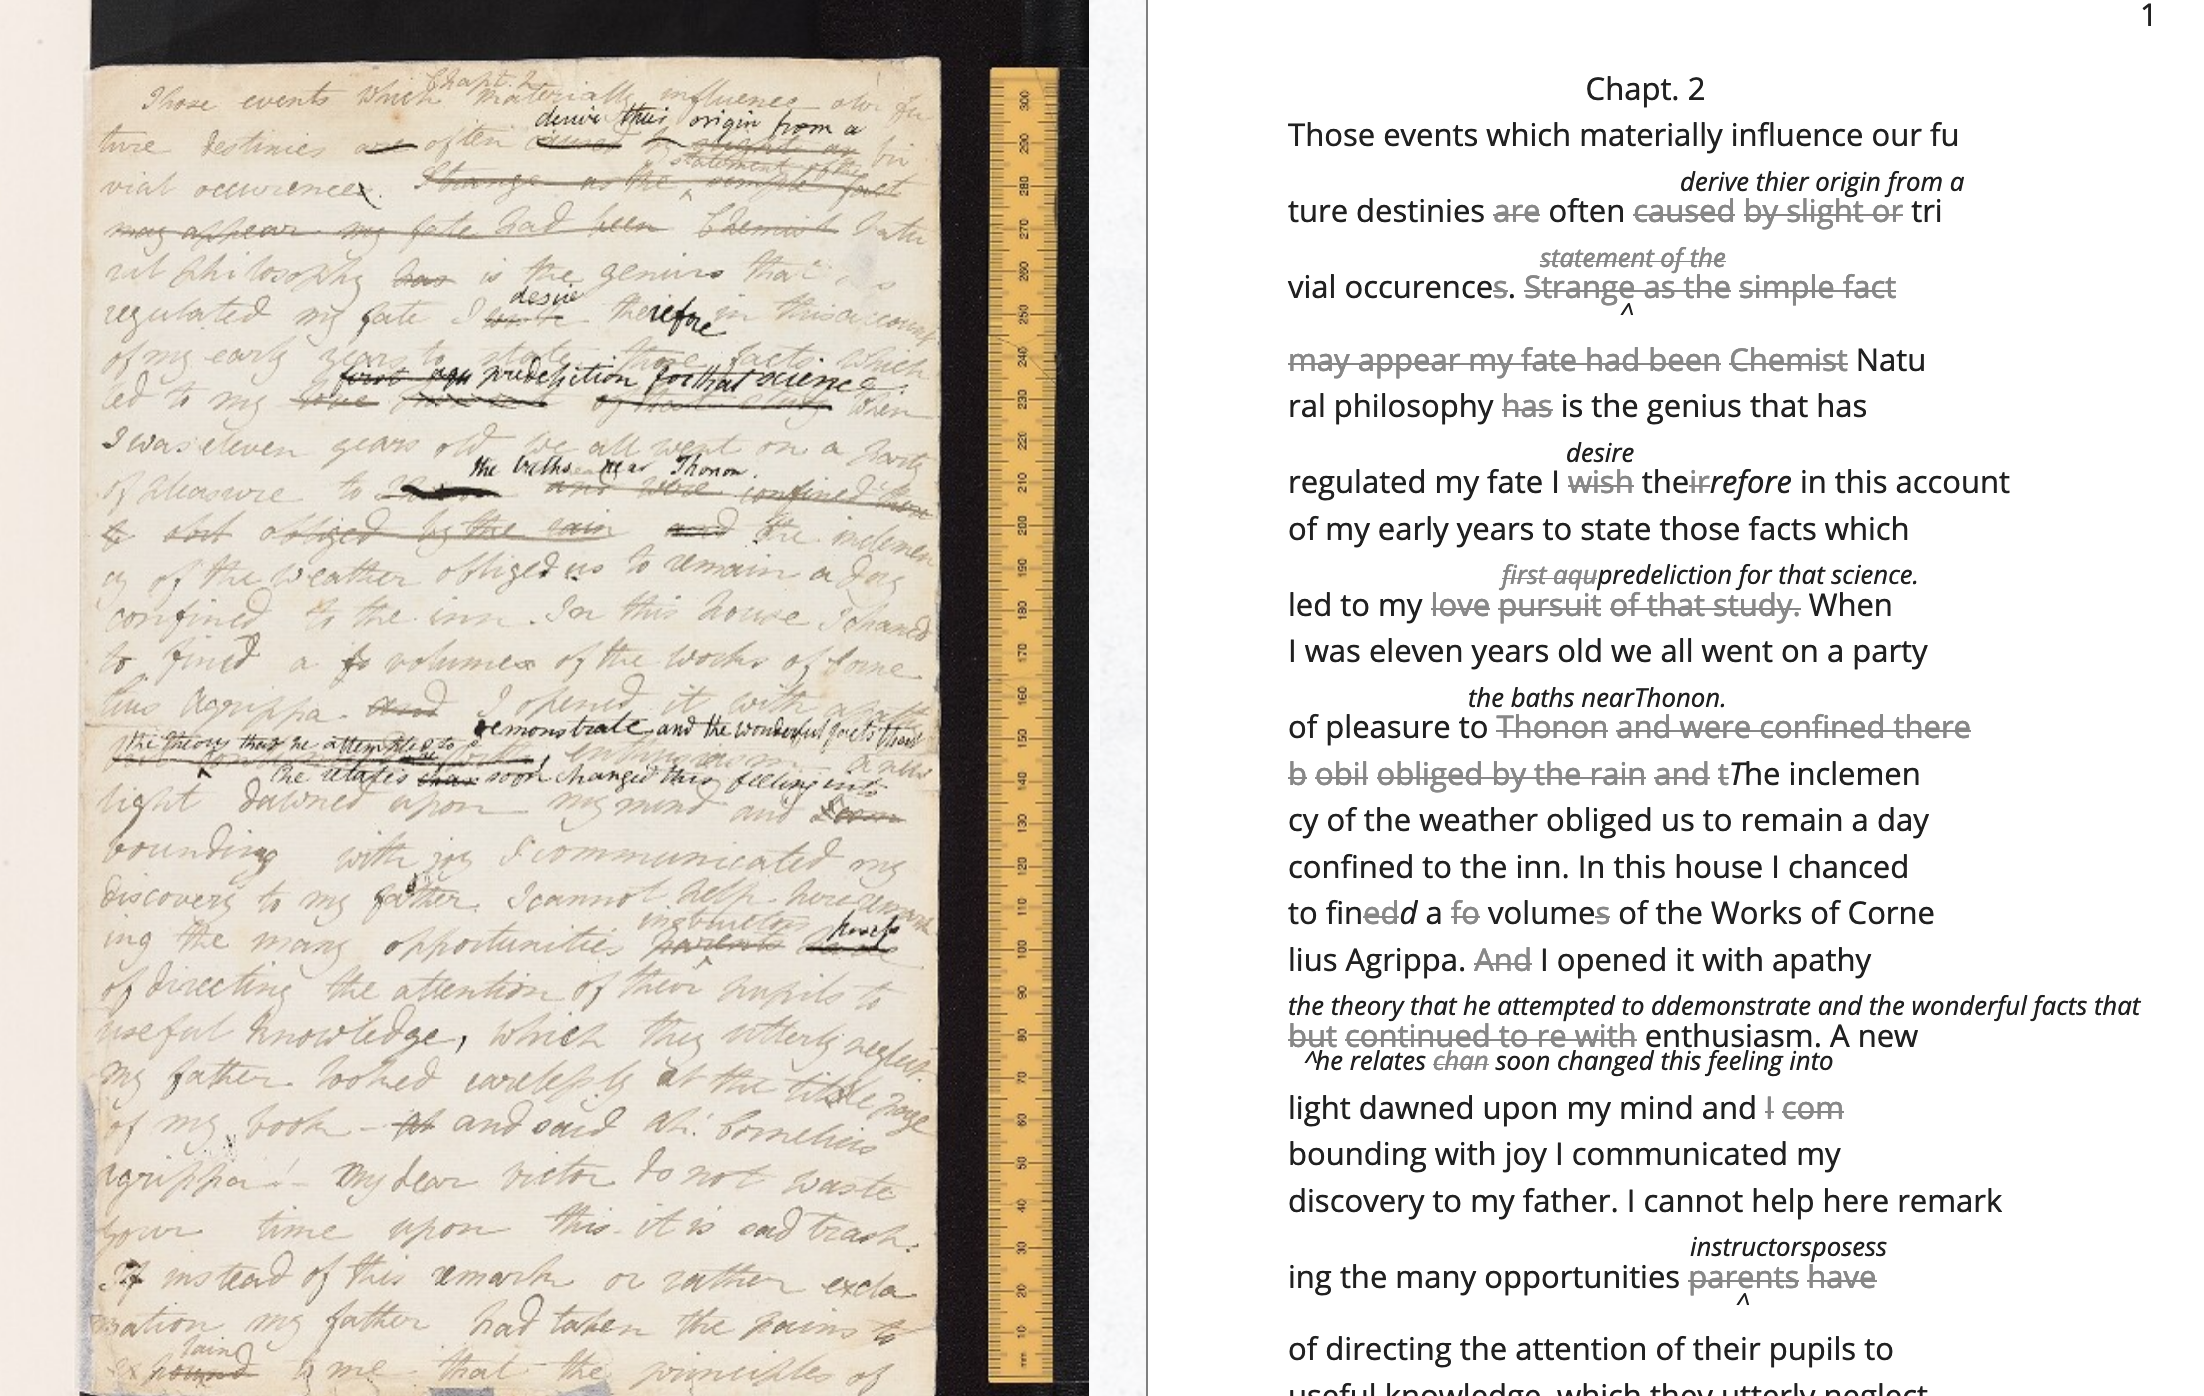
\includegraphics[width=.9\linewidth]{./sga_diplo.png}
\end{center}

Here is an excerpt of some of the TEI code underlying this page. Note
that the first few lines of the text contained within the \texttt{<line>}
tags:

\begin{SOURCE}
<line>Those events which materially influence our fu</line>
<line>ture destinies 
<del rend="strikethrough">are</del> often 
<mod>
    <del rend="strikethrough">caused</del>
    <del rend="strikethrough">by slight or</del>
    <add hand="\#pbs" place="superlinear">derive thier origin from
    a</add>
  </mod> tri
</line>
<line>vial occurence
<del rend="strikethrough">s</del>. 
<mod spanTo="\#c56-0005.01"/>
<del rend="strikethrough" next="\#c56-0005.02">Strange as the</del>
\end{SOURCE}

When scholars might simply scan and upload images of text, why would
they to go through the trouble of marking up a text with TEI? One
reason is that TEI facilitates deep and complex search of textual
material. For example, in the \emph{Frankenstein} project, the encoding
includes information about who is writing which portions of the
text. As 


For example, \emph{The Willa Cather Archive}, a digital archive
of the author's novels, stories, nonfiction, letters, and journalism,
offers both high-quality scanned images and encoded text of the same
works. In Cather's correspondance, one can see the benefit of the
TEI, which allows Here, a seemingly simple search tool reveals a precision and
complexity get with just a direct transcription or
scanned images.

Besides encoding text for searching, you might provide a diplomatic transcription, reproducing the typography the manuscript original, or encode editorial and authorial changes to a text over time. Because TEI is built to be customizable, many projects develop their own standards based on one of the existing guidelines, tailoring them to capture the key features of their source text.

\subsection{My customization of the TEI}
\label{sec:orge0e273e}
\subsection{Some engagement with Queer Theory}
\label{sec:orgf774655}
\section{commands}
\label{sec:orga6ef030}
c-c c-x f => create a new footnote
c-u c-c c-x f then select sort then renumber footnotes

block quotes: \#+BEGIN\(_{\text{QUOTE}}\) \& \#+END\(_{\text{QUOTE}}\)
\end{document}
